%% LyX 2.3.7 created this file.  For more info, see http://www.lyx.org/.
%% Do not edit unless you really know what you are doing.
\documentclass[english]{article}
\usepackage{mathpazo}
\usepackage[T1]{fontenc}
\usepackage[latin9]{inputenc}
\usepackage{geometry}
\geometry{verbose,tmargin=2cm,bmargin=2cm,lmargin=2cm,rmargin=2cm}
\usepackage{float}
\usepackage{amsmath}
\usepackage{amsthm}
\usepackage{amssymb}
\usepackage{graphicx}
\usepackage{setspace}

\makeatletter
%%%%%%%%%%%%%%%%%%%%%%%%%%%%%% Textclass specific LaTeX commands.
\numberwithin{equation}{section}
\numberwithin{figure}{section}

\makeatother

\usepackage{babel}
\begin{document}
\title{\doublespacing{}Electricity and Magnetism\linebreak{}
Tufts University\linebreak{}
Graduate School of Arts and Sciences\linebreak{}
Long Assignment 1\linebreak{}

\includegraphics{Lockups/A&S_Hori_BK+BL}}
\author{Jose Emmanuel Flores}
\date{October 11th, 2023}

\maketitle
\textbf{Statement of the problem.}

A small mass of the photon would be responsible for changing the Coulomb\textquoteright s
law from its classical form to 
\begin{equation}
\overrightarrow{F}=\frac{1}{4\pi\epsilon_{0}}\frac{q_{1}q_{2}}{r^{2}}\left(1+\frac{r}{\lambda}\right)\exp\left(\frac{-r}{\lambda}\right)\hat{r}\label{eq:Force}
\end{equation}
where $\lambda$ is a new constant of nature proportional to the inverse
of the photon mass ($mg^{-1}$). Assuming that the superposition principle
still holds, this formula can be easily generalized to any charge
distribution $\rho$. We will use this to reformulate Plimton \& Lawton\textquoteright s
experiments in terms of the small-photon-mass potential. 
\begin{enumerate}
\item Find the potential of a point charge $q$ situated at the origin of
the coordinate system, if we set the reference to be null at infinity,
assuming this new version of Coulomb\textquoteright s law.
\item If this charge $q$ is rather distributed on a conducting shell of
radius $R$ maintained at a constant potential value by a battery,
show that the potential at any point inside the shell at a distance
$r<R$ from the center satisfies:
\[
\frac{V(r)-V\left(R\right)}{V\left(R\right)}\approx\frac{-1}{6\lambda^{2}}\left[R^{2}-r^{2}\right]
\]
\item The other approach, subject of this problem, does not assume any specific
expression for the deviation of the electrostatic potential from Coulomb\textquoteright s
law. It is therefore more general, but less explicative. It only assumes
that the deviation to the Coulomb\textquoteright s potential is very
small, i.e. that:
\[
V\left(r\right)=kqr^{-\left(1+\epsilon\right)},\text{ with }\epsilon\ll1.
\]
Measuring the potential difference between two concentric spherical
shells, the outer shell of a radius $R$ being maintained at a constant
potential $V(R)$, and the inner shell of radius $r$ being initially
grounded, would test this hypothesis. Show that a small deviation
with respect to Coulomb\textquoteright s potential would yield a ratio
of the potential difference to the applied voltage of:
\[
\frac{V(r)-V\left(R\right)}{V\left(R\right)}=\frac{\epsilon}{2}\left[\ln\left(\frac{R-r}{R+r}\right)+\ln\left(\frac{4R^{2}}{R^{2}-r^{2}}\right)\right].
\]
\item The two approaches have been formulated in similar terms and can now
be compared. In 1970, Barnett et al. obtained a limit of $|\epsilon|<1.3\times10^{-13}$
using the generic deviation approach. How would Barnett limit on $\epsilon$
convert to a limit on $1/\lambda$? To answer this, assume that the
inner sphere has a radius of 60 cm, 2/3 of the radius of the large
sphere. Compare this result with the best limits on $\lambda$. Discuss
your comparison. This comparison shows that while being very general,
the second approach is not the most precise way to test all possible
assumptions about deviations to $1/r^{2}$.
\end{enumerate}
\textbf{Solutions.}

\textbf{1. }Let's start by write the equation (\ref{eq:Force}) as
\[
\overrightarrow{F}=q_{1}\overrightarrow{E},
\]
where 
\begin{equation}
\overrightarrow{E}=\frac{1}{4\pi\epsilon_{0}}\frac{q_{2}}{r^{2}}\left(1+\frac{r}{\lambda}\right)\exp\left(\frac{-r}{\lambda}\right)\hat{r},\label{eq:EField}
\end{equation}
in the previous expresion let's make the following change of variables
\[
q_{2}\rightarrow q,\frac{r}{\lambda}\rightarrow x\implies\frac{1}{r^{2}}=\frac{1}{\lambda^{2}x^{2}},dr=\lambda dx
\]
then we have that the electric field given in equation (\ref{eq:EField})
becomes 
\[
\overrightarrow{E}=\frac{1}{4\pi\epsilon_{0}}\frac{q}{\lambda^{2}x^{2}}\left(1+x\right)\exp\left(-x\right)\hat{r.}
\]
On the other hand, we know that the potential can be obtain by the
following expression 
\[
V(r)=-\int_{\mathcal{O}}^{r}\overrightarrow{E}\cdot d\overrightarrow{l},
\]
 but because $\overrightarrow{E}$ is a central force, the previous
integral can be written as 
\[
V(r)=-\int_{\mathcal{O}}^{r}Edr,
\]
then, we have that 
\[
V=-\frac{1}{4\pi\epsilon_{0}}\frac{q}{\lambda}\int_{\mathcal{O}}^{r}\frac{1}{x^{2}}\left(1+x\right)\exp\left(-x\right)dx,
\]
then if we rename 
\[
\alpha=\frac{1}{4\pi\epsilon_{0}}\frac{q}{\lambda},
\]
we have that the previous integral, can be written as 
\[
V=-\alpha\int\left(\frac{1}{x^{2}}+\frac{1}{x}\right)\exp\left(-x\right)dx,
\]
\begin{equation}
V=-\alpha\left(\int\frac{1}{x^{2}}\exp\left(-x\right)dx+\int\frac{1}{x}\exp\left(-x\right)dx\right),\label{eq:VPotential}
\end{equation}
and the problem nos transforms in solving the following two integrals
\[
\int\frac{1}{x^{2}}\exp\left(-x\right)dx\hspace{1em}\text{,}\int\frac{1}{x}\exp\left(-x\right)dx,
\]
but now, let's focus on the first integral, 
\begin{equation}
\int\frac{1}{x^{2}}\exp\left(-x\right)dx,\label{eq:Intx2Exp(x)}
\end{equation}
and the plan will be to attack it using integration by parts, and
choose 
\[
dv=\frac{1}{x^{2}}dx\implies v=-\frac{1}{x},
\]
and 
\[
u=\exp\left(-x\right)\implies du=-\exp\left(-x\right)dx,
\]
then, we have that the equation (\ref{eq:Intx2Exp(x)}) will be 
\[
\int\frac{1}{x^{2}}\exp\left(-x\right)dx=-\frac{1}{x}\exp\left(-x\right)-\int\left(-\frac{1}{x}\right)\left(-\exp\left(-x\right)dx\right),
\]
\[
\implies\int\frac{1}{x^{2}}\exp\left(-x\right)dx=-\frac{1}{x}\exp\left(-x\right)-\int\frac{1}{x}\exp\left(-x\right)dx.
\]
And if we know plug this new information in the equation (\ref{eq:VPotential}),
we have that 
\[
V=-\alpha\left(-\frac{1}{x}\exp\left(-x\right)-\int\frac{1}{x}\exp\left(-x\right)dx+\int\frac{1}{x}\exp\left(-x\right)dx\right),
\]
and as we can see, the integrals cancel, then, we have that 
\[
V=\alpha\frac{1}{x}\exp\left(-x\right),
\]
or in the original coordinates, we have that 
\[
V\left(r\right)=\frac{\alpha}{\left(\frac{r}{\lambda}\right)}\exp\left(-\frac{r}{\lambda}\right)=\frac{\alpha\lambda}{r}\exp\left(-\frac{r}{\lambda}\right),
\]
\[
\implies V\left(r\right)=\frac{\alpha\lambda}{r}\exp\left(-\frac{r}{\lambda}\right),
\]
but in the previous expression we need to evaluate on the limits of
integration, which are the observation point $\mathcal{O}$ and $r$,
which I intentionally droped from the calculation, just to make the
notiation a little bit cleaner. Even more, because we are considering
our reference point at $\infty$, we have that the exponential goes
to $0$, and then, we have 
\[
V\left(r\right)=\frac{\alpha\lambda}{r}\exp\left(-\frac{r}{\lambda}\right),
\]
and using the actual representation of $\alpha$, we have 
\[
V\left(r\right)=\frac{1}{4\pi\epsilon_{0}}\frac{q}{r}\exp\left(-\frac{r}{\lambda}\right).
\]

\textbf{2. }For this part we're going to generalize the previous result
to a continuous distribution, in this particular case, a spherical
shell, and for that, we're going to use the following diagram.
\begin{figure}[H]
\begin{centering}
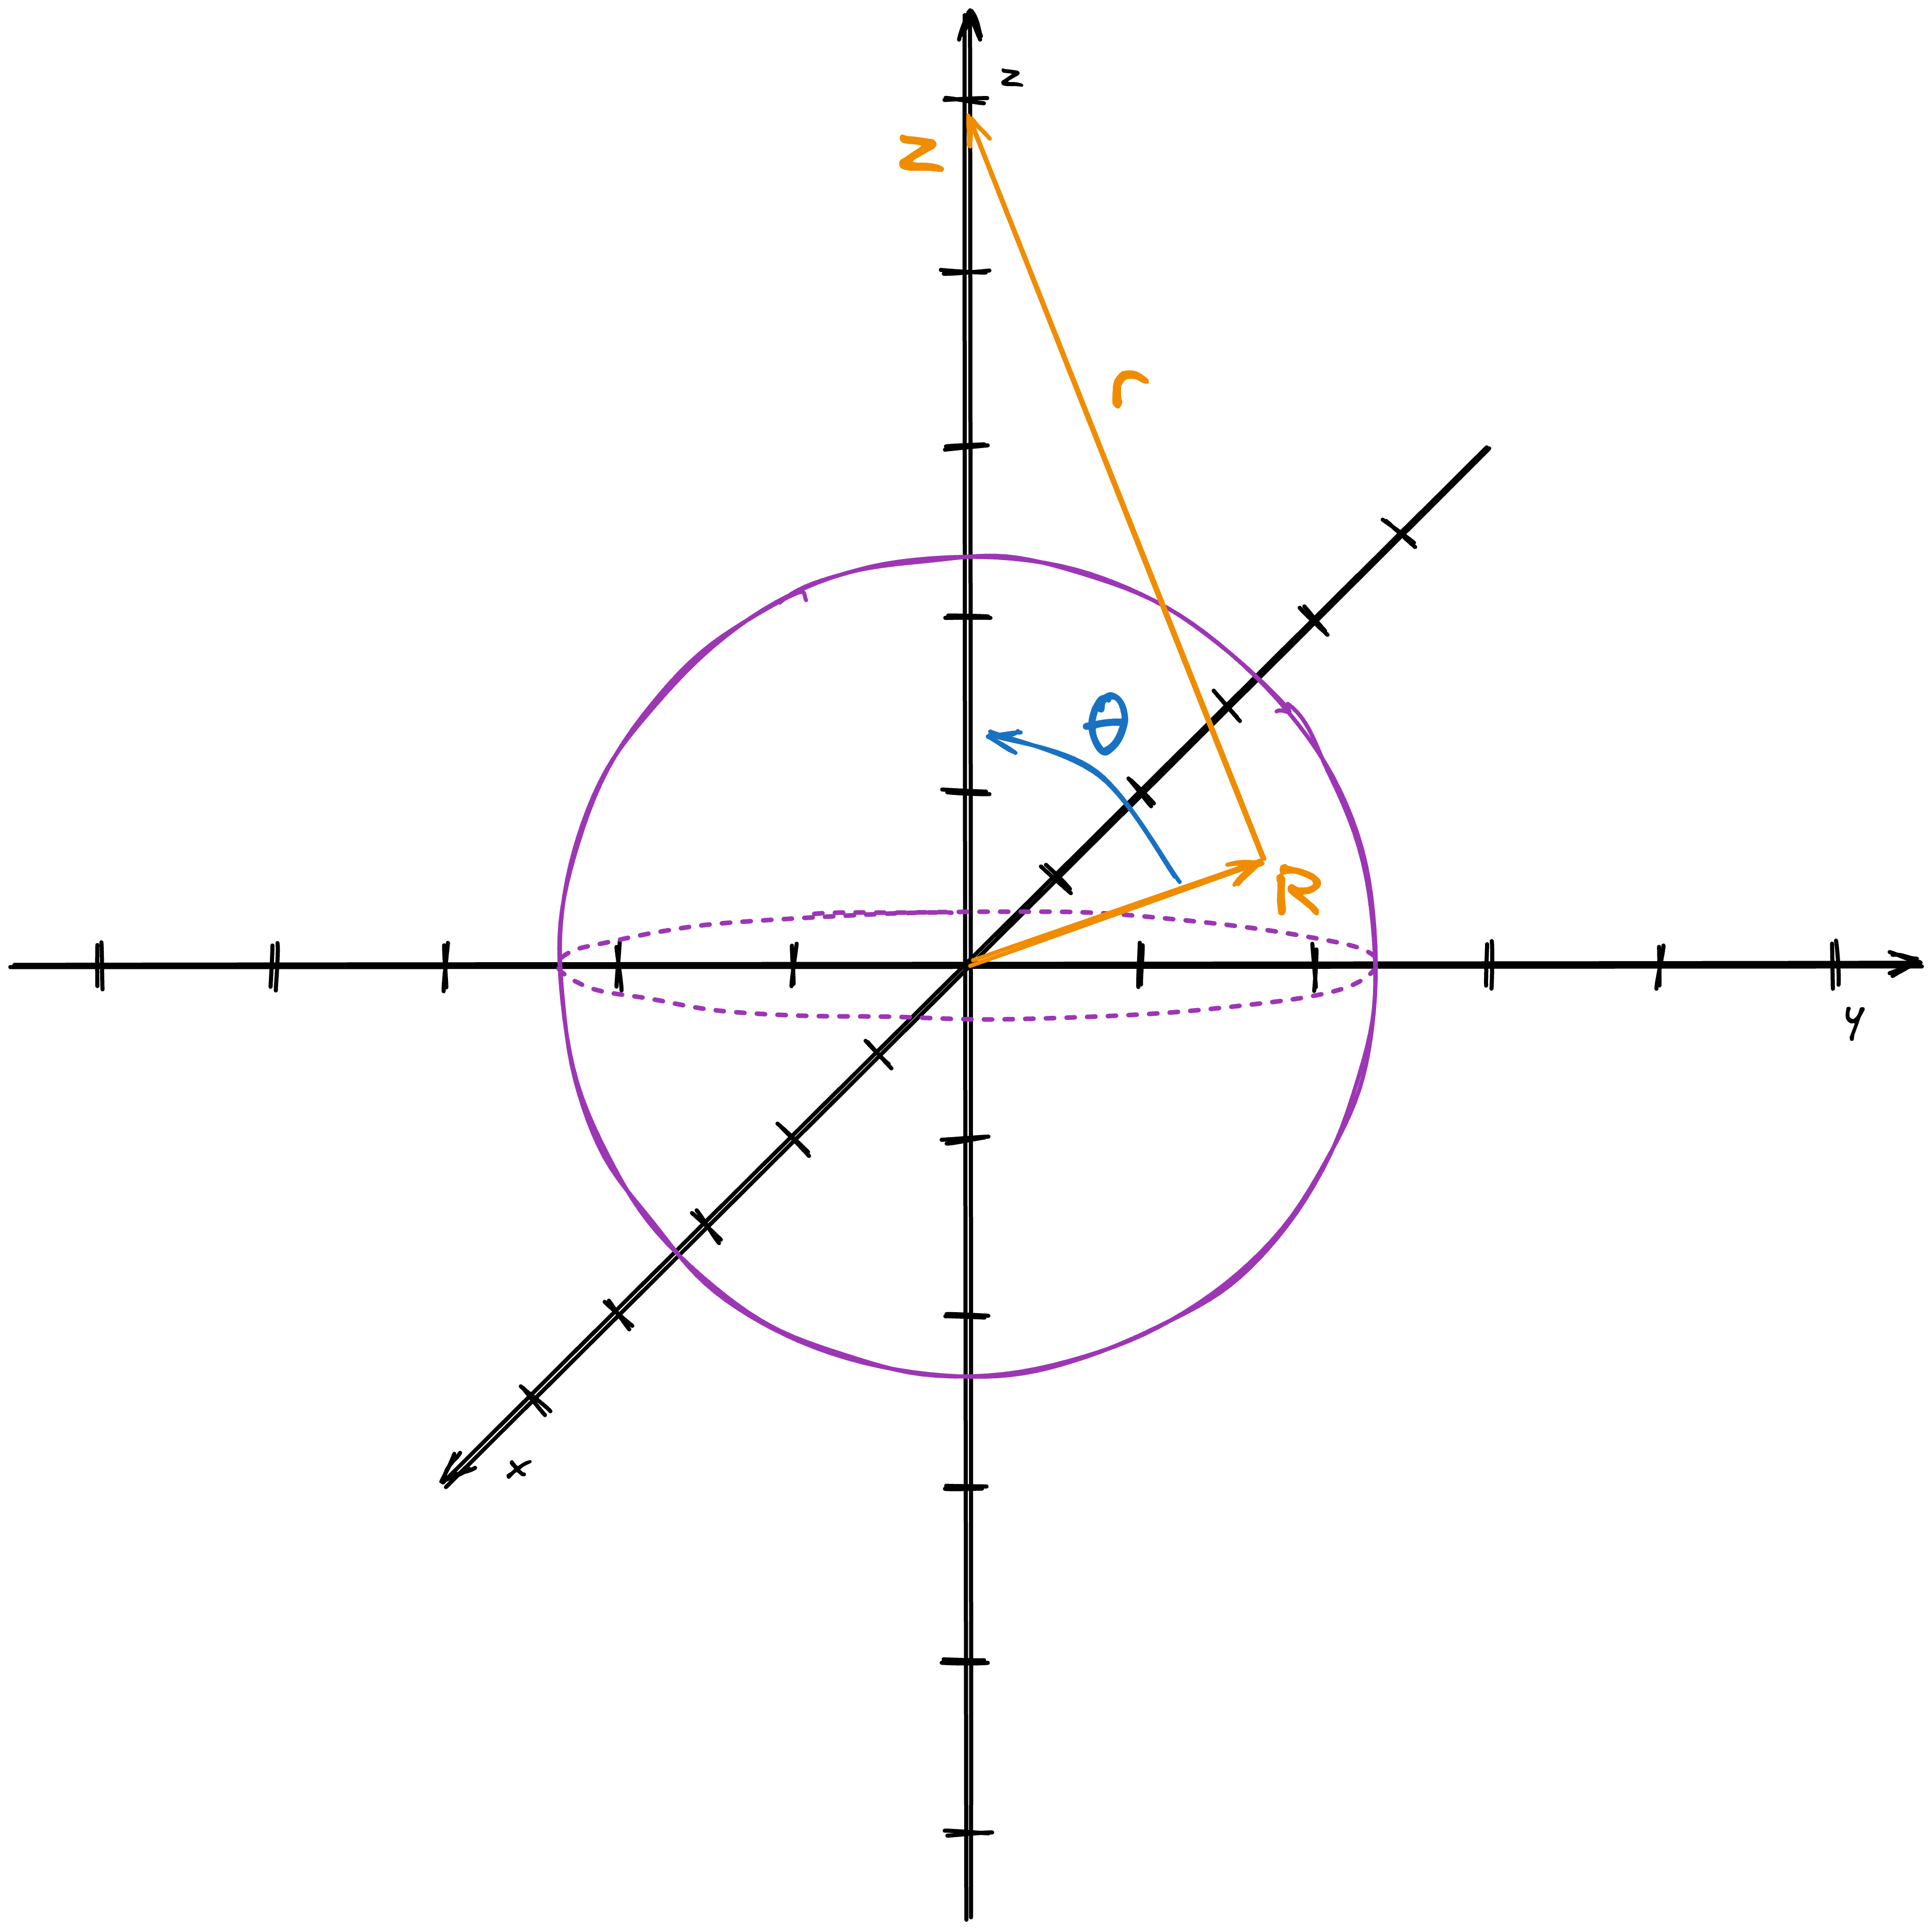
\includegraphics[scale=0.05]{Shell}\caption{Spherical shell with constant surface density.}
\par\end{centering}
\end{figure}
Therefore, we have that 
\[
dq=\sigma dS,
\]
where $\sigma$ it's a surface charge density, thus 
\[
dV=\frac{1}{4\pi\epsilon_{0}r}\exp\left(-\frac{r}{\lambda}\right)\sigma dS,
\]
\[
\implies V=\int_{S}\frac{1}{4\pi\epsilon_{0}r}\exp\left(-\frac{r}{\lambda}\right)\sigma dS,
\]
in this case, given the geometry, we have that 
\[
V=\frac{\sigma}{4\pi\epsilon_{0}}\int_{S}\frac{1}{r}\exp\left(-\frac{r}{\lambda}\right)dS,
\]
now let's write the explicit integral and also the differential surface
element 
\[
V=\frac{\sigma}{4\pi\epsilon_{0}}\int_{0}^{2\pi}\int_{0}^{\pi}\frac{1}{r}\exp\left(-\frac{r}{\lambda}\right)R^{2}\sin\theta d\theta d\phi,
\]
but because there's no dependence of $\phi$ in the integrand, that
integration becomes immediate 
\[
V=\frac{\sigma R^{2}}{2\epsilon_{0}}\int_{0}^{\pi}\frac{1}{r}\exp\left(-\frac{r}{\lambda}\right)\sin\theta d\theta,
\]
but given the geometry of this problem, we have that 
\[
r=\sqrt{R^{2}+z^{2}-2Rz\cos\theta},
\]
therefore, we can write the integral as 
\[
V=\frac{\sigma R^{2}}{2\epsilon_{0}}\int_{0}^{\pi}\frac{\exp\left(-\frac{1}{\lambda}\sqrt{R^{2}+z^{2}-2Rz\cos\theta}\right)}{\sqrt{R^{2}+z^{2}-2Rz\cos\theta}}\sin\theta d\theta.
\]
So let's try to write the previous equation in a better way, and for
so, let's make the following change of variable 
\[
u=\sqrt{R^{2}+z^{2}-2Rz\cos\theta},
\]
\[
\implies\frac{du}{d\theta}=\frac{2Rz\sin\theta}{\sqrt{R^{2}+z^{2}-2Rz\cos\theta}},
\]
\[
\implies du=\frac{2Rz\sin\theta}{\sqrt{R^{2}+z^{2}-2Rz\cos\theta}}d\theta,
\]
and then we have that 
\[
\frac{du}{2Rz}=\frac{\sin\theta}{\sqrt{R^{2}+z^{2}-2Rz\cos\theta}}d\theta,
\]
therefore, the whole integral tranforms into 
\[
V=\frac{\sigma R^{2}}{2\epsilon_{0}}\int_{0}^{\pi}\frac{\exp\left(-\frac{1}{\lambda}\sqrt{R^{2}+z^{2}-2Rz\cos\theta}\right)}{\sqrt{R^{2}+z^{2}-2Rz\cos\theta}}\sin\theta d\theta=\frac{\sigma R^{2}}{2\epsilon_{0}}\frac{1}{2Rz}\int_{b}^{b}\exp\left(-\frac{u}{\lambda}\right)du,
\]
\[
\therefore V=\frac{\sigma}{4\epsilon_{0}}\frac{R}{z}\int_{b}^{b}\exp\left(-\frac{u}{\lambda}\right)du,
\]
and the above integral it's immediate, thus, we have 
\[
V=\frac{\sigma}{4\epsilon_{0}}\frac{R}{z}\left[-\lambda\exp\left(-\frac{1}{\lambda}\sqrt{R^{2}+z^{2}-2Rz\cos\theta}\right)\right]_{0}^{\pi},
\]
\[
\implies V=-\lambda\frac{\sigma}{4\epsilon_{0}}\frac{R}{z}\left[\exp\left(-\frac{1}{\lambda}\sqrt{R^{2}+z^{2}+2Rz}\right)-\exp\left(-\frac{1}{\lambda}\sqrt{R^{2}+z^{2}-2Rz}\right)\right],
\]
\[
\implies V=-\lambda\frac{\sigma}{4\epsilon_{0}}\frac{R}{z}\left[\exp\left(-\frac{1}{\lambda}\sqrt{\left(R+z\right)^{2}}\right)-\exp\left(-\frac{1}{\lambda}\sqrt{\left(R-z\right)^{2}}\right)\right],
\]
and because we're considering the case in which we're inside the sphere,
we have that $R-z>0$, then
\[
\implies V\left(z\right)=-\lambda\frac{\sigma}{4\epsilon_{0}}\frac{R}{z}\left[\exp\left(-\frac{R+z}{\lambda}\right)-\exp\left(-\frac{R-z}{\lambda}\right)\right],
\]
and before move on to more calculations let's rename make the following
change of variable 
\[
\alpha=\frac{\sigma}{4\epsilon_{0}},
\]
therefore, the potential field becomes 
\[
V\left(z\right)=\alpha\frac{\lambda R}{z}\left[\exp\left(\frac{z-R}{\lambda}\right)-\exp\left(\frac{-z-R}{\lambda}\right)\right].
\]
On the other hand, with this result we can obtain $V\left(R\right)$,
which will be 
\[
V\left(R\right)=\alpha\lambda\left[1-\exp\left(-\frac{2R}{\lambda}\right)\right].
\]
And now, let's Taylor Expand the exponentials inside the potential
field, but before doing any math, let's write the first three terms
of the Taylor expansion for an exponential function 
\[
\exp\left(x\right)\approx1+x+\frac{1}{2!}x^{2}+\frac{1}{3!}x^{3}.
\]
So, for the $\exp\left(\frac{z-R}{\lambda}\right)$ we have 
\[
\exp\left(\frac{z-R}{\lambda}\right)\approx1+\left(\frac{z-R}{\lambda}\right)+\frac{1}{2!}\left(\frac{z-R}{\lambda}\right)^{2}+\frac{1}{3!}\left(\frac{z-R}{\lambda}\right)^{3}+\dots,
\]
and, for the other exponential, we have 
\[
\exp\left(\frac{-z-R}{\lambda}\right)\approx1+\left(\frac{-z-R}{\lambda}\right)+\frac{1}{2!}\left(\frac{-z-R}{\lambda}\right)^{2}+\frac{1}{3!}\left(\frac{-z-R}{\lambda}\right)^{3}+\dots,
\]
and now, let's take the rest of the two previous equations, and let's
do it term by term separatedly 
\[
\left(\frac{z-R}{\lambda}\right)-\left(\frac{-z-R}{\lambda}\right)=\frac{2z}{\lambda},
\]
\[
\frac{1}{2!}\left[\left(\frac{z-R}{\lambda}\right)^{2}-\left(\frac{-z-R}{\lambda}\right)^{2}\right]=\frac{1}{2!}\left(\frac{-4zR}{\lambda^{2}}\right),
\]
\[
\frac{1}{3!}\left[\left(\frac{z-R}{\lambda}\right)^{3}-\left(\frac{-z-R}{\lambda}\right)^{3}\right]=\frac{1}{3!}\left[\left(\frac{z-R}{\lambda}\right)^{3}+\left(\frac{z+R}{\lambda}\right)^{3}\right]=\frac{1}{3!}\left(\frac{6R^{2}z}{\lambda^{3}}+\frac{2z^{3}}{\lambda^{3}}\right),
\]
and now, let's add the previous three equations together 
\[
\mathcal{O}_{3}=\frac{2z}{\lambda}+\frac{1}{2!}\left(\frac{-4zR}{\lambda^{2}}\right)+\frac{1}{3!}\left(\frac{6R^{2}z}{\lambda^{3}}+\frac{2z^{3}}{\lambda^{3}}\right),
\]
\[
\implies\mathcal{O}_{3}=\frac{2z}{\lambda}-\frac{2zR}{\lambda^{2}}+\frac{R^{2}z}{\lambda^{3}}+\frac{2z^{3}}{6\lambda^{3}},
\]
$\implies$therefore the potential field will be 
\[
V\left(z\right)_{\mathcal{O}_{3}}=\alpha\frac{\lambda R}{z}\left[\frac{2z}{\lambda}-\frac{2zR}{\lambda^{2}}+\frac{R^{2}z}{\lambda^{3}}+\frac{z^{3}}{3\lambda^{3}}\right]=\alpha\left[2R-\frac{2R^{2}}{\lambda}+\frac{R^{3}}{\lambda^{3}}+\frac{2Rz^{2}}{6\lambda^{3}}\right],
\]
\[
\implies V\left(z\right)_{\mathcal{O}_{3}}=\alpha\left[2R-\frac{2R^{2}}{\lambda}+\frac{R^{3}}{\lambda^{2}}+\frac{2Rz^{2}}{6\lambda^{2}}\right],
\]
on the other, hand, we can also consider an aproximation for the potential
$V\left(R\right)$, and we have that 
\[
V\left(R\right)_{\mathcal{O}_{3}}=\alpha\lambda\left[1-\left(1+\left(-\frac{2R}{\lambda}\right)+\frac{1}{2!}\left(-\frac{2R}{\lambda}\right)^{2}+\frac{1}{3!}\left(-\frac{2R}{\lambda}\right)^{3}\right)\right],
\]
\[
\implies V\left(R\right)_{\mathcal{O}_{3}}=\alpha\lambda\left[\frac{2R}{\lambda}-\frac{4R}{2\lambda^{2}}^{2}+\frac{8R^{3}}{6\lambda^{3}}\right],
\]
\[
\therefore V\left(R\right)_{\mathcal{O}_{3}}=\alpha\left[2R-\frac{2R}{\lambda}^{2}+\frac{4R^{3}}{3\lambda^{2}}\right],
\]
and with this result, we have that 
\[
V\left(z\right)_{\mathcal{O}_{3}}-V\left(R\right)_{\mathcal{O}_{3}}=\alpha\left[2R-\frac{2R^{2}}{\lambda}+\frac{R^{3}}{\lambda^{2}}+\frac{2Rz^{2}}{6\lambda^{2}}-2R+\frac{2R^{2}}{\lambda}-\frac{4R^{3}}{3\lambda^{2}}\right],
\]
\[
\implies V\left(z\right)_{\mathcal{O}_{3}}-V\left(R\right)_{\mathcal{O}_{3}}=\alpha\left[-\frac{R^{3}}{3\lambda^{2}}+\frac{2Rz^{2}}{6\lambda^{2}}\right]=\alpha R\left[\frac{2z^{2}}{6\lambda^{2}}-\frac{2R^{2}}{6\lambda^{2}}\right],
\]
\[
\therefore V\left(z\right)_{\mathcal{O}_{3}}-V\left(R\right)_{\mathcal{O}_{3}}=\frac{2\alpha R}{6\lambda^{2}}\left[z^{2}-R^{2}\right],
\]
and, with this result we have 
\[
\frac{V\left(z\right)_{\mathcal{O}_{3}}-V\left(R\right)_{\mathcal{O}_{3}}}{V\left(R\right)_{\mathcal{O}_{3}}}=\frac{\frac{2\alpha R}{6\lambda^{2}}\left[z^{2}-R^{2}\right]}{\alpha\left[2R-\frac{2R}{\lambda}^{2}+\frac{4R^{3}}{3\lambda^{2}}\right]}=\frac{\frac{2\alpha R}{6\lambda^{2}}\left[z^{2}-R^{2}\right]}{2\alpha R\left[1-\frac{R}{\lambda}+\frac{2R^{2}}{3\lambda^{2}}\right]},
\]
\[
\implies\frac{V\left(z\right)_{\mathcal{O}_{3}}-V\left(R\right)_{\mathcal{O}_{3}}}{V\left(R\right)_{\mathcal{O}_{3}}}=\frac{1}{6\lambda^{2}}\frac{\left[z^{2}-R^{2}\right]}{\left[1-\frac{R}{\lambda}+\frac{2R^{2}}{3\lambda^{2}}\right]},
\]
in the previous equation we can perform another aproximation for the
denominator, we can perform a binomial-like expansion in order to
transform the denominator into the numerator, but with this we're
going to have something like 
\[
\frac{1}{\left[1-\frac{R}{\lambda}+\frac{2R^{2}}{3\lambda^{2}}\right]}\approx1+\frac{R}{\lambda}+\mathcal{O}\left(\frac{1}{\lambda^{3}}\right),
\]
then, we have 
\[
\frac{V\left(z\right)_{\mathcal{O}_{3}}-V\left(R\right)_{\mathcal{O}_{3}}}{V\left(R\right)_{\mathcal{O}_{3}}}=\frac{1}{6\lambda^{2}}\left[z^{2}-R^{2}\right]\left[1+\frac{R}{\lambda}+\mathcal{O}\left(\frac{1}{\lambda^{3}}\right)\right],
\]
but in the previous expression we have terms that behave like $1/\lambda^{3}$,
therefore, we drop those terms, and we keep up to order $1/\lambda^{2}$,
then we finnlay have 
\[
\frac{V\left(z\right)_{\mathcal{O}_{3}}-V\left(R\right)_{\mathcal{O}_{3}}}{V\left(R\right)_{\mathcal{O}_{3}}}=\frac{1}{6\lambda^{2}}\left[z^{2}-R^{2}\right]=-\frac{1}{6\lambda^{2}}\left[R^{2}-z^{2}\right],
\]
\begin{equation}
\therefore\frac{V(r)-V\left(R\right)}{V\left(R\right)}\approx-\frac{1}{6\lambda^{2}}\left[R^{2}-z^{2}\right]
\end{equation}

\textbf{3. }For this part, we should have that the potential for a
point charge is given as 
\[
V_{p}\left(r\right)=kqr^{-\left(1+\epsilon\right)},
\]
where $\epsilon\ll1$, and the sub index $p$ s just to make even
more explicit that this potential it's for a point charge. So the
first thing is to generalize the given potential for a continous distribution,
in this case, let's generalize it to a spherical shell. And before
doing any calculation, let's use the following diagram as a guide
\begin{figure}[H]
\centering{}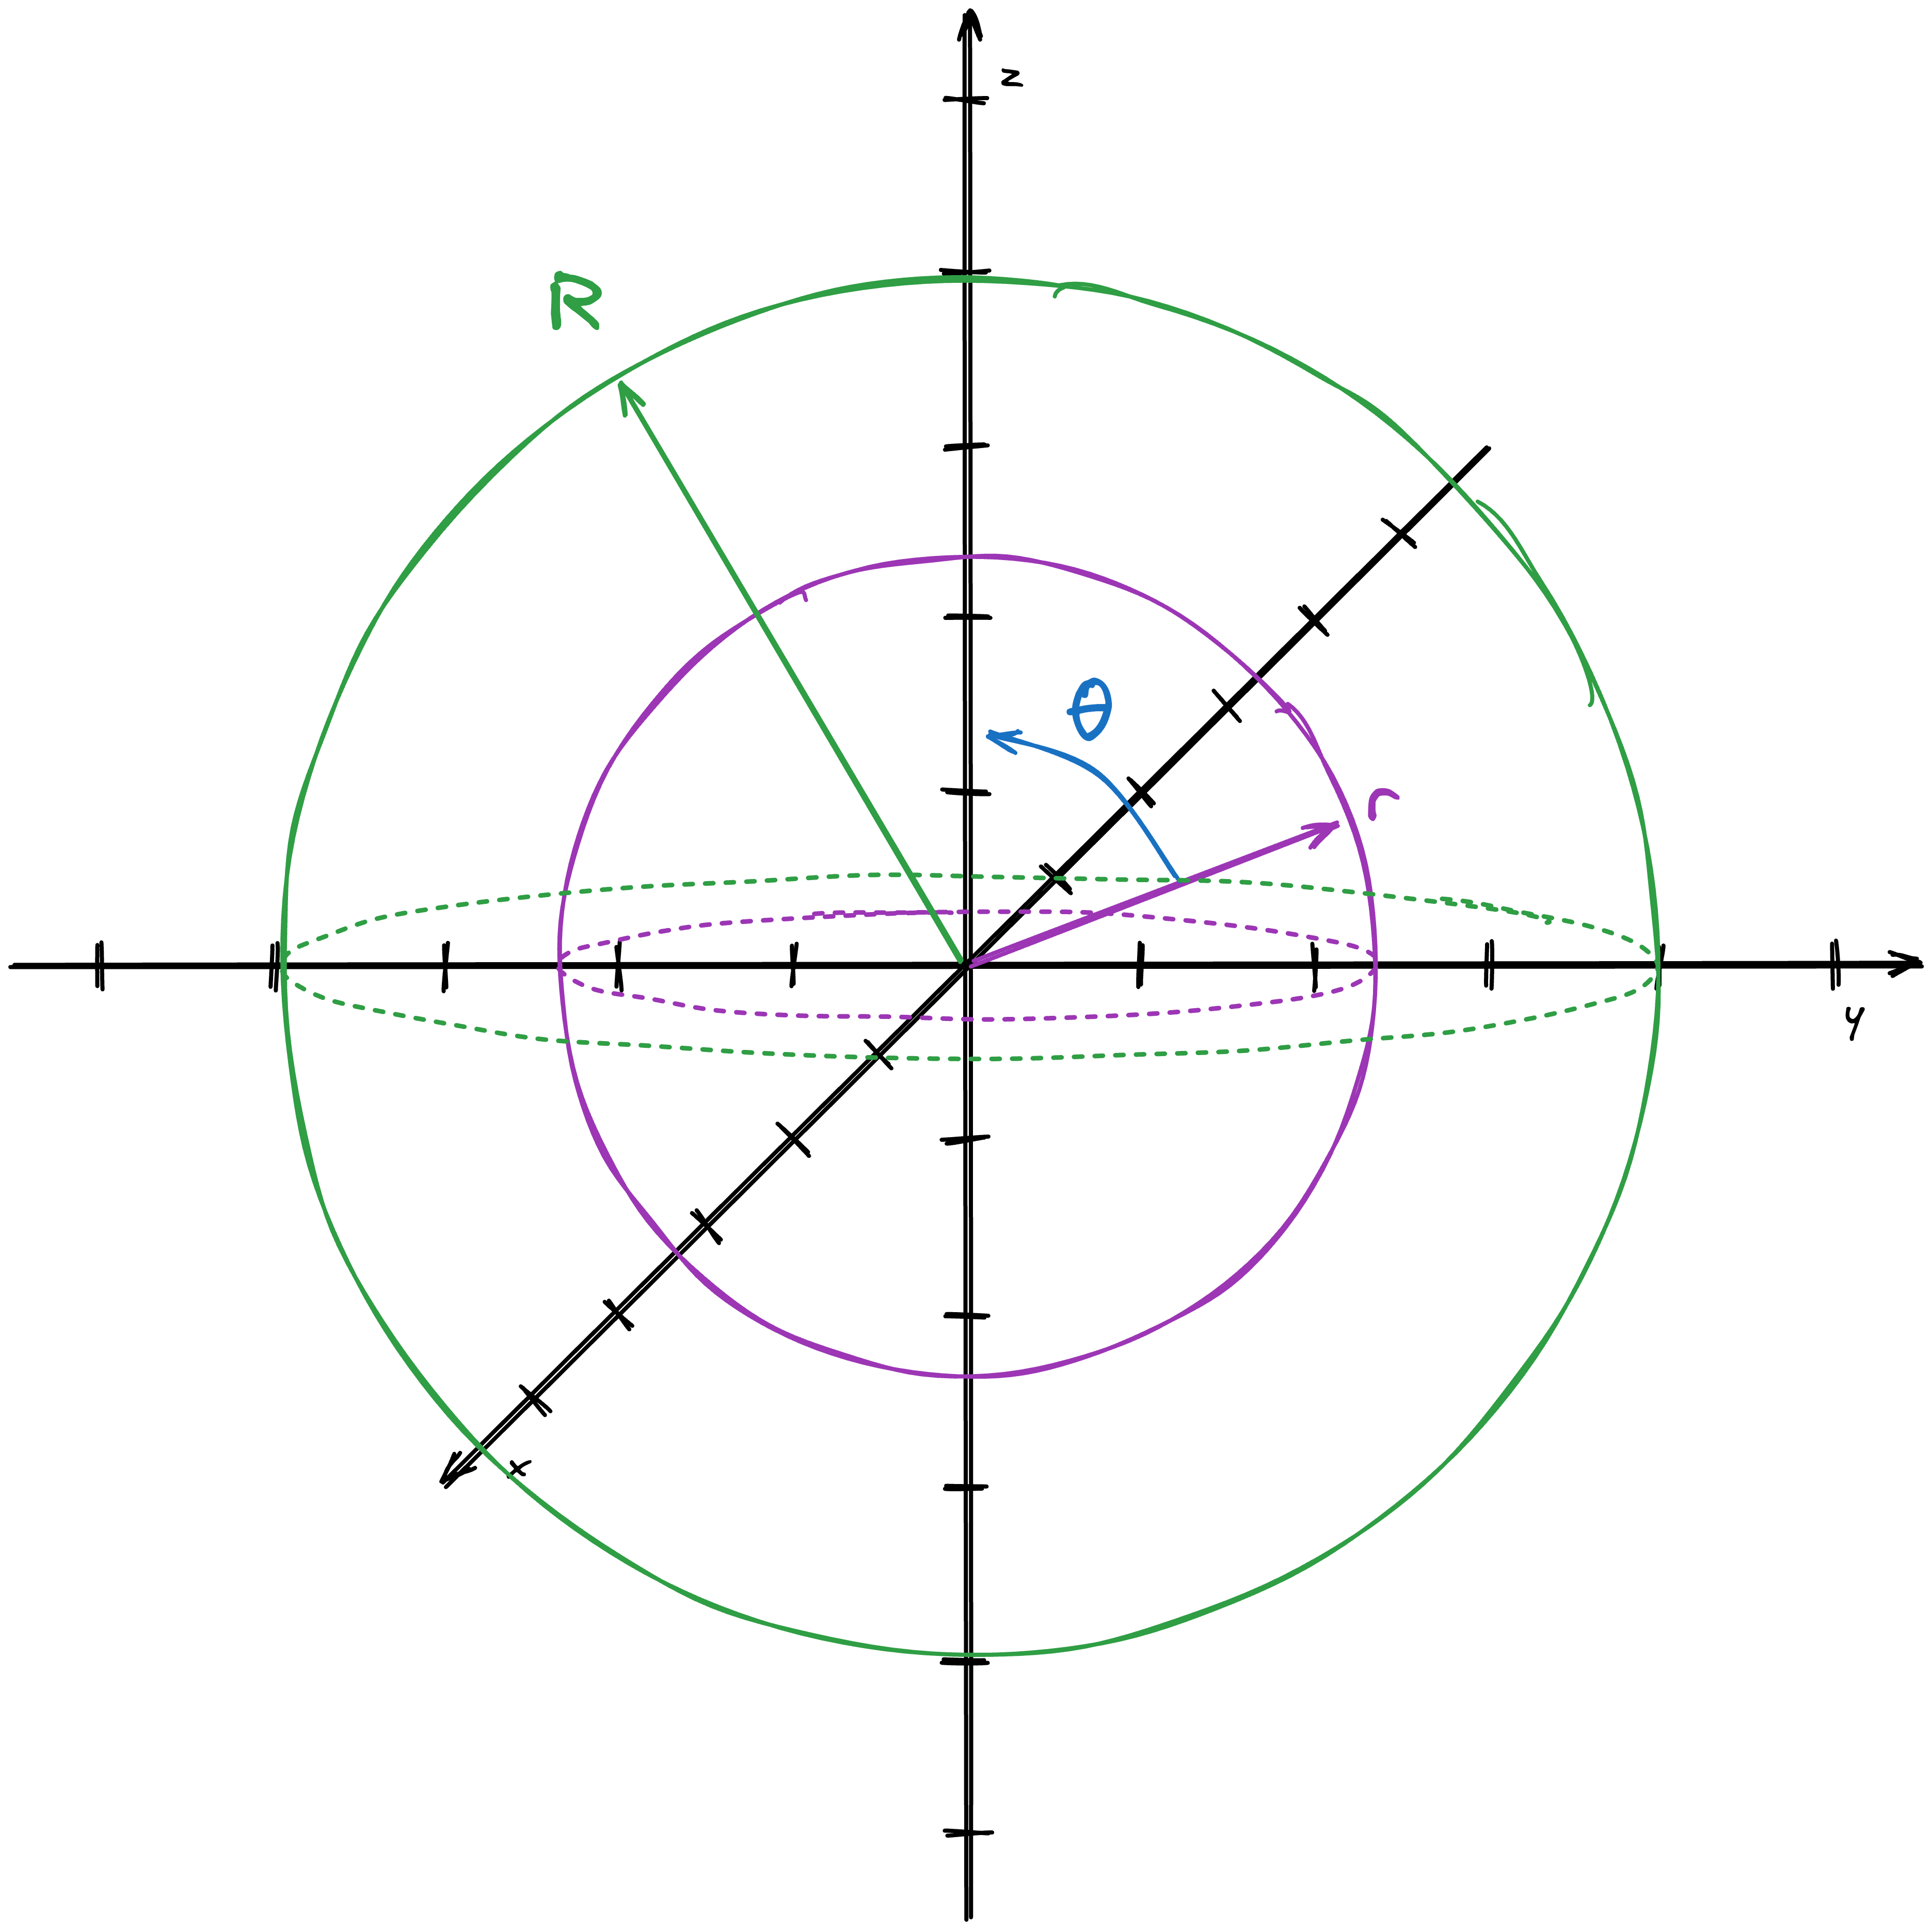
\includegraphics[scale=0.1]{ConcentricShells}\caption{Concentric shells.}
\end{figure}
What we're going to do is to integrate the previous expression for
a surface, i.e, 
\[
V=\int_{S}V_{p}dS,
\]
where $dS=R^{2}\sin\theta d\theta d\phi,$ and we also have to consider
this $dq=\sigma dS$, therefore, we have 
\[
V=\int_{S}k\sigma r^{-\left(1+\epsilon\right)}R^{2}\sin\theta d\theta d\phi,
\]
and from the figure we can see that 
\[
r^{2}=z^{2}+R^{2}-2zR\cos\theta,
\]
therefore, we have that 
\[
V=k\sigma\int_{0}^{2\pi}d\phi\int_{0}^{\pi}\frac{R^{2}\sin\theta d\theta}{\left(z^{2}+R^{2}-2zR\cos\theta\right)^{\left(1+\epsilon\right)}},
\]
and now, for this integral we're going to use the following change
of variables 
\[
u^{2}=z^{2}+R^{2}-2zR\cos\theta,
\]
\[
\implies2udu=2zR\sin\theta d\theta,
\]
\[
\implies udu=zR\sin\theta d\theta,
\]
\[
\implies\sin\theta d\theta=\frac{1}{zR}udu
\]
and with change of variables we have that $\theta=0$, implies $u=R-z$,
and $u=\pi$, implies $u=R+z$, thus, we have that 
\[
V=k\sigma\frac{R^{2}}{zR}\int_{0}^{2\pi}d\phi\int_{R-z}^{R+z}\frac{udu}{u^{\left(1+\epsilon\right)}},
\]
\[
\implies V=k\sigma\frac{2\pi R}{z}\int_{R-r}^{R+r}\frac{udu}{u^{\left(1+\epsilon\right)}}=\frac{k\sigma}{zR}\frac{1}{1-\epsilon}\left(u^{\left(1-\epsilon\right)}\right)|_{R-r}^{R+r},
\]
\[
\implies V=k\sigma\frac{2\pi R}{z}\frac{1}{1-\epsilon}\left(u^{\left(1-\epsilon\right)}\right)|_{R-r}^{R+r},
\]
\[
\therefore V\left(r\right)=\frac{\alpha R}{r\left(1-\epsilon\right)}\left(\left(R+r\right)^{\left(1-\epsilon\right)}-\left(R-r\right)^{\left(1-\epsilon\right)}\right),
\]
where $\alpha=2\pi k\sigma$, and if we know evaluate $V\left(R\right)$,
we have that 
\[
V\left(R\right)=\alpha\frac{R}{R}\frac{1}{1-\epsilon}\left(\left(R+R\right)^{\left(1-\epsilon\right)}-\left(R-R\right)^{\left(1-\epsilon\right)}\right)=\frac{\alpha}{1-\epsilon}\left(2R\right)^{1-\epsilon},
\]
\[
\implies V\left(R\right)=\frac{\alpha}{1-\epsilon}\left(2R\right)^{1-\epsilon}.
\]
Therefore 
\[
\frac{V\left(r\right)}{V\left(R\right)}=\frac{\frac{\alpha R}{r\left(1-\epsilon\right)}\left(\left(R+r\right)^{\left(1-\epsilon\right)}-\left(R-r\right)^{\left(1-\epsilon\right)}\right)}{\frac{\alpha}{1-\epsilon}\left(2R\right)^{1-\epsilon}},
\]
\[
\implies\frac{V\left(r\right)}{V\left(R\right)}=\frac{R}{r}\frac{\left(\left(R+r\right)^{\left(1-\epsilon\right)}-\left(R-r\right)^{\left(1-\epsilon\right)}\right)}{\left(2R\right)^{1-\epsilon}}.
\]
Now, if we use the following approximation $x^{1-\epsilon}=x\left(1-\ln x\right)$,
then we have that 
\[
\left(2R\right)^{1-\epsilon}=2R\left(1-\ln2R\right),
\]
and also 
\[
\left(R+r\right)^{\left(1-\epsilon\right)}=\left(R+r\right)\left(1-\epsilon\ln\left(R+r\right)\right),
\]
\[
\left(R-r\right)^{1-\epsilon}=\left(R-r\right)\left(1-\epsilon\ln\left(R-r\right)\right),
\]
then we can express 
\[
\frac{V\left(r\right)}{V\left(R\right)}=\frac{R}{r}\frac{\left(\left(R+r\right)\left(1-\epsilon\ln\left(R+r\right)\right)-\left(R-r\right)\left(1-\epsilon\ln\left(R-r\right)\right)\right)}{2R\left(1-\epsilon\ln2R\right)},
\]
\[
\implies\frac{V\left(r\right)}{V\left(R\right)}=\frac{1}{2r}\frac{\left(\left(R+r\right)\left(1-\epsilon\ln\left(R+r\right)\right)-\left(R-r\right)\left(1-\epsilon\ln\left(R-r\right)\right)\right)}{\left(1-\epsilon\ln2R\right)},
\]
now, let's play a little with the numerator of the previous equation,
which, for a better reading, I'm going to call it $D$, then 
\[
D=R+r-R\epsilon\ln\left(R+r\right)-r\epsilon\ln\left(R+r\right)-R+r+R\epsilon\ln\left(R-r\right)-r\epsilon\ln\left(R-r\right),
\]
then, we have 
\[
D=2r+R\epsilon\left(\ln\left(R+r\right)-\ln\left(R-r\right)\right)-r\epsilon\left(\ln\left(R+r\right)+\ln\left(R-r\right)\right),
\]
but using properties of the logatimic function, we can write the previous
equation as 
\[
D=2r+R\epsilon\left(\ln\frac{R+r}{R-r}\right)-r\epsilon\left(\ln\left[\left(R+r\right)\left(R-r\right)\right]\right),
\]

\[
\implies D=2r+R\epsilon\left(\ln\frac{R+r}{R-r}\right)-r\epsilon\left(\ln\left(R^{2}-r^{2}\right)\right),
\]
\[
\implies D=2r+R\epsilon\left(\ln\frac{R+r}{R-r}\right)+r\epsilon\left(\ln\left(R^{2}-r^{2}\right)^{-1}\right),
\]
\[
\therefore D=2r+R\epsilon\left(\ln\frac{R+r}{R-r}\right)+r\epsilon\left(\ln\frac{1}{R^{2}-r^{2}}\right)
\]
then the expression, becomes 
\[
\frac{V\left(r\right)}{V\left(R\right)}=\frac{1}{2r}\frac{2r+R\epsilon\left(\ln\frac{R+r}{R-r}\right)+r\epsilon\left(\ln\frac{1}{R^{2}-r^{2}}\right)}{\left(1-\epsilon\ln2R\right)},
\]
and now, in order to get rid of the denominator, we're going to perform
the following approximation, for $x$ small enough, we have 
\[
\frac{1}{1-x}\approx1+x,
\]
then, we can express the denominator as 
\[
\frac{1}{1-\epsilon\ln2R}\approx1+\epsilon\ln2R,
\]
therefore, we have that 
\[
\frac{V\left(r\right)}{V\left(R\right)}\approx\frac{1}{2r}\left(2r+R\epsilon\left(\ln\frac{R+r}{R-r}\right)+r\epsilon\left(\ln\frac{1}{R^{2}-r^{2}}\right)\right)\left(1+\epsilon\ln2R\right),
\]
\[
\implies\frac{V\left(r\right)}{V\left(R\right)}\approx\left(1+\frac{R\epsilon}{2r}\left(\ln\frac{R+r}{R-r}\right)+\frac{\epsilon}{2}\left(\ln\frac{1}{R^{2}-r^{2}}\right)\right)\left(1+\epsilon\ln2R\right)
\]
but becasue $\epsilon\ll1$ we are not going to consider the terms
that go as $\epsilon^{2}$, then, we have that the previous expression
can be written as 
\[
\frac{V\left(r\right)}{V\left(R\right)}\approx1+\frac{R\epsilon}{2r}\left(\ln\frac{R+r}{R-r}\right)+\frac{\epsilon}{2}\left(\ln\frac{1}{R^{2}-r^{2}}\right)+\epsilon\ln2R,
\]
but we can write the last term as 
\[
\epsilon\ln2R=\frac{\epsilon}{2}2\ln2R=\frac{\epsilon}{2}\ln\left(2R\right)^{2}=\frac{\epsilon}{2}\ln\left(4R^{2}\right),
\]
\[
\implies\epsilon\ln2R=\frac{\epsilon}{2}\ln\left(4R^{2}\right),
\]
therefore, we have that 
\[
\frac{V\left(r\right)}{V\left(R\right)}\approx1+\frac{R\epsilon}{2r}\left(\ln\frac{R+r}{R-r}\right)+\frac{\epsilon}{2}\left(\ln\frac{1}{R^{2}-r^{2}}\right)+\frac{\epsilon}{2}\ln\left(4R^{2}\right),
\]
and again, using the properties of the logaritmic function, we have
\[
\frac{V\left(r\right)}{V\left(R\right)}\approx1+\frac{R\epsilon}{2r}\left(\ln\frac{R+r}{R-r}\right)+\frac{\epsilon}{2}\left(\ln\frac{4R^{2}}{R^{2}-r^{2}}\right),
\]
\[
\implies\frac{V\left(r\right)}{V\left(R\right)}-1\approx\frac{\epsilon}{2}\left[\frac{R}{r}\left(\ln\frac{R+r}{R-r}\right)+\left(\ln\frac{4R^{2}}{R^{2}-r^{2}}\right)\right],
\]
\[
\therefore\frac{V\left(r\right)-V\left(R\right)}{V\left(R\right)}\approx\frac{\epsilon}{2}\left[\frac{R}{r}\left(\ln\frac{R+r}{R-r}\right)+\left(\ln\frac{4R^{2}}{R^{2}-r^{2}}\right)\right].
\]

\textbf{4. }For this final question we have to compare the two approximations,
and one way to do it is by comparing the expressions for the potentials,
on one hand we have 
\[
\frac{V(r)-V\left(R\right)}{V\left(R\right)}\approx\frac{-1}{6\lambda^{2}}\left[R^{2}-r^{2}\right],
\]
and on another 
\[
\frac{V(r)-V\left(R\right)}{V\left(R\right)}=\frac{\epsilon}{2}\left[\frac{R}{r}\ln\left(\frac{R-r}{R+r}\right)+\ln\left(\frac{4R^{2}}{R^{2}-r^{2}}\right)\right],
\]
and now, if we have that $r=\frac{2}{3}R$, then, form the first equation
we have 
\[
\frac{V(r)-V\left(R\right)}{V\left(R\right)}\approx\frac{-1}{6\lambda^{2}}\left[R^{2}-\frac{4}{9}R^{2}\right]=-\frac{1}{6\lambda^{2}}\left(\frac{5}{9}R^{2}\right),
\]
and on the other hand, for the second approximation we have that 
\[
\frac{V(r)-V\left(R\right)}{V\left(R\right)}=\frac{\epsilon}{2}\left[\frac{3}{2}\ln\left(\frac{R}{5R}\right)+\ln\left(\frac{4R^{2}}{\frac{5}{9}R^{2}}\right)\right]=\frac{\epsilon}{2}\left[\ln\left(\frac{R}{5R}\right)+\ln\left(\frac{36R}{5R}\right)\right]
\]
\[
\implies\frac{V(r)-V\left(R\right)}{V\left(R\right)}=\frac{\epsilon}{2}\left[\ln\left(\frac{1}{5}\right)+\ln\left(\frac{36}{5}\right)\right],
\]
then if we compare the two expressions for the potential, we have
that 
\[
-\frac{1}{6\lambda^{2}}\left(\frac{5}{9}R^{2}\right)=\frac{\epsilon}{2}\left[\frac{3}{2}\ln\left(\frac{1}{5}\right)+\ln\left(\frac{36}{5}\right)\right],
\]
and if we solve for $1/\lambda$, we have that 
\[
-\frac{1}{6\lambda^{2}}=\frac{\epsilon}{2}\frac{\left[\frac{3}{2}\ln\left(\frac{1}{5}\right)+\ln\left(\frac{36}{5}\right)\right]}{\left(\frac{5}{9}R^{2}\right)},
\]
\[
\implies\left(\frac{1}{\lambda}\right)^{2}=-\frac{3\epsilon\left[\ln\left(\frac{1}{5}\right)+\ln\left(\frac{36}{5}\right)\right]}{\left(\frac{5}{9}R^{2}\right)}=-3\epsilon\left(\frac{-0.440076}{5/9R^{2}}\right),
\]
\[
\implies\left(\frac{1}{\lambda}\right)^{2}=\frac{2.37641}{\left(0.6\right)^{2}}\epsilon,
\]
but $\epsilon<1.3\times10^{-13}$, then, we have that 
\[
\frac{1}{\lambda}=\sqrt{\left(\frac{2.38}{\left(0.6\right)^{2}}\right)\left(1.3\times10^{-13}\right)},
\]
\[
\implies\frac{1}{\lambda}=9.27062\times10^{-7}m^{-1}.
\]

\end{document}
